In this chapter, we provide an overview of the fundamental concepts and equations that underpin the field of cosmology following textbooks \citet{2003moco.book.....D} and \citet{2008cosm.book.....W}.

\section{Einstein Field Equations}
The Einstein Field Equations are the fundamental equations of General Relativity, describing how matter and energy influence the curvature of spacetime. Introduced by \citet{1915SPAW.......844E}, these equations extend Newton's law of universal gravitation to a relativistic context, accounting for the effects of high velocities and strong gravitational fields.

The EFE establish a relationship between the geometry of spacetime and the distribution of matter within it. They are expressed with the metric $g_{\mu\nu}$, which describes the curvature of spacetime, and the stress-energy tensor $T_{\mu\nu}$, which characterizes the distribution of matter and energy. The EFE are given by:
\begin{equation}
    G_{\mu\nu} + \Lambda g_{\mu\nu}= \frac{8\pi G}{c^4} T_{\mu\nu},
    \label{eq:einstein_field_equations}
\end{equation}
where $\Lambda$ is the cosmological constant, $G$ is the gravitational constant, and $c$ is the speed of light. The Einstein tensor $G_{\mu\nu}$ is defined by:
\begin{equation}
    G_{\mu\nu} = R_{\mu\nu} - \frac{1}{2} R g_{\mu\nu},
    \label{eq:einstein_tensor}
\end{equation}
the $R_{\mu\nu}$ is the Riemann tensor, described by the Christoffel symbols $\Gamma^\lambda_{\mu\nu}$ as:
\begin{equation}
    R_{\mu\nu} = \partial_\lambda \Gamma^\lambda_{\mu\nu} - \partial_\nu \Gamma^\lambda_{\mu\lambda} + \Gamma^\lambda_{\lambda\sigma} \Gamma^\sigma_{\mu\nu} - \Gamma^\lambda_{\mu\sigma} \Gamma^\sigma_{\lambda\nu},
    \label{eq:ricci_curvature_tensor}
\end{equation}
the Ricci scalar $R$ is given by:
\begin{equation}
    R = g^{\mu\nu} R_{\mu\nu},
    \label{eq:ricci_scalar}
\end{equation}
Assuming a perfect fluid as the source of the gravitational field, the stress-energy tensor is given by
\begin{equation}
    T_{\mu\nu} = \left(\rho + p \right) u_{\mu} u_{\nu} + p g_{\mu\nu},
    \label{eq:stress_energy_tensor}
\end{equation}
where \( \rho \) is the energy density, \( p \) is the pressure, and \( u_{\mu} \) is the four-velocity of the fluid.
In a homogeneous and isotropic universe, \( u_{\mu} \) is given by
\begin{equation}
    u_{\mu} = (-c, 0, 0, 0),
    \label{eq:four_velocity}
\end{equation}
Therefore, each component of the stress-energy tensor can be expressed as
\begin{equation}
    T_{00} = \rho c^2, \quad T_{ij} = p g_{ij},
    \label{eq:stress_energy_components}
\end{equation}
Different speices of matter and energy contribute to the energy density \( \rho \) and pressure \( P \) in the universe. The equation of state parameter \( w \) is defined as the ratio of pressure \( P \) to energy density \( \rho \):
\begin{equation}
    w = \frac{p}{\rho}.
    \label{eq:equation_of_state}
\end{equation}
For perfect fluids, the equation of state parameter can be derived by considering the trace of the stress-energy tensor:
\begin{equation}
    0 = T = g^{\mu\nu} T_{\mu\nu} = (\rho + p)(-1) + 4p = -\rho + 3p,
    \label{eq:stress_energy_trace}
\end{equation}
For non-relativistic matter where $p = 0$, the equation of state parameter is \( w = 0 \). 
For cosmological constant, the equation of state parameter can be derived by comparing the effective stress-energy of the cosmological constant $T_{\mu\nu}^{(\Lambda)} = \rho_{\Lambda} g_{\mu\nu}$ to the stress-energy tensor of a perfect fluid:
\begin{align}
    \rho_{\Lambda} &= \frac{\Lambda c^4}{8\pi G} \label{eq:lambda_density} \\
    \left(\rho_{\Lambda} + p_{\Lambda} \right) u_{\mu} u_{\nu} + p_{\Lambda} g_{\mu\nu} &= T_{\mu\nu}^{(\Lambda)} = \rho_{\Lambda} g_{\mu\nu}  \\
    \rho_{\Lambda} + p_{\Lambda} &= 0 \quad \text{(valid for all $\mu$, $\nu$)} \nonumber \\
    p_{\Lambda} &= -\rho_{\Lambda} \label{eq:lambda_pressure}
\end{align}
Therefore, the equation of state parameter for cosmological constant is \( w = -1 \).

To summarize, the Equation os States for each component of the universe are:
\begin{equation}
    w = 
    \begin{cases}
        0 & \text{fatter}, \\
        \frac{1}{3} & \text{Radiation}, \\
        -1 & \text{Cosmological Constant}.
    \end{cases}
    \label{eq:equation_of_state_summary}
\end{equation}

In realistic universe, the energy density and pressure are contributed by multiple components. Assuming the interaction between different components is negligible, the total stress-energy tensor is the sum of the individual stress-energy tensors:
\begin{equation}
    T_{\mu\nu} = \sum_i (T_i)_{\mu\nu},
\end{equation}
where \( i \) denotes the different components of the universe. Therefore, the total energy density and pressure are given by:
\begin{equation}
    \rho = \sum_i \rho_i, \quad p = \sum_i p_i.
\end{equation}
In the late universe, where each component evolves adiabatically, the energy density scales as:
\begin{equation}
    \rho_i \propto a^{-3(1 + w_i)},
    \label{eq:energy_density_scaling}
\end{equation}
where \( a \) is the scale factor, and \( w_i \) is the equation of state parameter for the \( i \)-th component. 

\section{FLRW Metric and the Friedmann Equations}\label{sec:flrw_metric}
The Friedmann-Lemaître-Robertson-Walker (FLRW) metric describes a homogeneous and isotropic universe and is given by~\citet{1972gcpa.book.....W}:
\begin{equation}
    ds^2 = -c^2 dt^2 + a^2(t) \left[ d\chi^2 + f_K^2(\chi) \left( d\theta^2 + \sin^2\theta \, d\phi^2 \right) \right],
    \label{eq:flrw_metric}
\end{equation}
where \( a(t) \) is the scale factor, \( \chi \) is the comoving radial coordinate, and \( d\Omega^2 = d\theta^2 + \sin^2\theta \, d\phi^2 \) represents the metric on the unit two-sphere. The function \( f_K(\chi) \) encodes the spatial curvature of the universe and is defined as:
\begin{equation}
    f_K(\chi) = 
    \begin{cases}
        \dfrac{1}{\sqrt{-K}} \sinh\left(\sqrt{-K}\chi\right) & \text{for } K < 0, \\
        \chi & \text{for } K = 0, \\
        \dfrac{1}{\sqrt{K}} \sin\left(\sqrt{K}\chi\right) & \text{for } K > 0,
    \end{cases}
    \label{eq:fk_definition}
\end{equation}
where \( K \) is the spatial curvature constant, with \( K < 0 \) corresponding to an open universe, \( K = 0 \) to a flat universe, and \( K > 0 \) to a closed universe.

For the FLRW metric, the non-zero components of the Einstein tensor are:
\begin{align}
    G_{00} &= 3\left( \frac{\dot{a}}{a} \right)^{2} + 3\frac{K c^2}{a^2}, \label{eq:G00_component} \\
    G_{ij} &= -\left( 2\frac{\ddot{a}}{a} + \left( \frac{\dot{a}}{a} \right)^2 + \frac{K c^2}{a^2} \right) a^2 g_{ij}, \label{eq:Gij_component}
\end{align}
where the dot denotes differentiation with respect to cosmic time \( t \).

Substituting the components of \( G_{\mu\nu} \) and \( T_{\mu\nu} \) into the Einstein field equations~\eqref{eq:einstein_field_equations}, we obtain the Friedmann equations~\citep{1922ZPhy...10..377F}:
\begin{itemize}
    \item First Friedmann equation ($00$ component):
    \begin{equation}
        3 \left( \frac{\dot{a}}{a} \right)^2 + 3\frac{Kc^2}{a^2} + \Lambda c^2 = \frac{8\pi G}{c^4} \rho c^2
    \end{equation}
    \begin{equation}
        \left( \frac{\dot{a}}{a} \right)^2 = \frac{8\pi G}{3} \rho - \frac{Kc^2}{a^2} + \frac{\Lambda c^2}{3}
        \label{eq:friedmann_first}
    \end{equation}
    \item Second Friedmann equation ($ii$ component):
    \begin{equation}
        -\left(2\frac{\ddot{a}}{a} + \left( \frac{\dot{a}}{a} \right)^2 + \frac{Kc^2}{a^2}\right)g_{ii} + \Lambda c^2 g_{ii} = \frac{8\pi G}{c^4} P g_{ii}
    \end{equation}
    \begin{equation}
        \frac{\ddot{a}}{a} = -\frac{4\pi G}{c^4} P - \frac{1}{2} \left(\left( \frac{\dot{a}}{a} \right)^2 
            + \frac{Kc^2}{a^2} - \Lambda c^2 \right)
    \end{equation}
    \begin{equation}
        \frac{\ddot{a}}{a} = -\frac{4\pi G}{3} \left( \rho + \frac{3P}{c^2} \right) + \frac{\Lambda c^2}{3}
        \label{eq:friedmann_second}
    \end{equation}
\end{itemize}
Introducing the Hubble parameter \( H \) and the critical density \( \rho_c \), we can simplify the Friedmann equations. The Hubble parameter is defined as:
\begin{equation}
    H = \frac{\dot{a}}{a},
    \label{eq:hubble_parameter}
\end{equation}
and the critical density is defined as:
\begin{equation}
    \rho_c = \frac{3 H^2}{8\pi G}.
    \label{eq:critical_density}
\end{equation}
Substituting \( H \) and \( \rho_c \) into the first Friedmann equation~\eqref{eq:friedmann_first}, we obtain:
\begin{equation}
    H^2 = H^2 \frac{\rho}{\rho_c} - \frac{K c^2}{a^2} + \frac{\Lambda c^2}{3}.
    \label{eq:friedmann_with_critical_density}
\end{equation}
Rearranging terms, we get:
\begin{equation}
    1 = \frac{\rho}{\rho_c} - \frac{K c^2}{a^2 H^2} + \frac{\Lambda c^2}{3 H^2}.
    \label{eq:friedmann_normalized}
\end{equation}
Defining the density parameters:
\begin{equation}
    \Omega_m = \frac{\rho_m}{\rho_c}, \quad \Omega_r = \frac{\rho_r}{\rho_c}, \quad \Omega_\Lambda = \frac{\rho_\Lambda}{\rho_c} = \frac{\Lambda c^2}{3 H^2}, \quad \Omega_K = -\frac{K c^2}{a^2 H^2},
    \label{eq:density_parameters}
\end{equation}
where \( \rho_m \) and \( \rho_r \) are the energy densities of matter and radiation, respectively, and \( \rho_\Lambda \) is the effective energy density associated with the cosmological constant, we can write the first Friedmann equation as:
\begin{equation}
    1 = \Omega_r + \Omega_m + \Omega_K + \Omega_\Lambda.
    \label{eq:friedmann_density_parameters}
\end{equation}
The evolution of the density parameters with the scale factor \( a \) can be derived from the conservation of energy-momentum and the equations of state. For matter-dominated and radiation-dominated universes, the energy densities scale as:
\begin{equation}
    \rho_m \propto a^{-3}, \quad \rho_r \propto a^{-4}.
    \label{eq:energy_density_scaling}
\end{equation}
Therefore, the corresponding density parameters vary with \( a \) as:
\begin{equation}
    \Omega_m(a) = \Omega_{m0} a^{-3} \left( \frac{H_0}{H(a)} \right)^2, \quad \Omega_r(a) = \Omega_{r0} a^{-4} \left( \frac{H_0}{H(a)} \right)^2,
    \label{eq:density_parameters_evolution}
\end{equation}
where the subscript \( 0 \) denotes present-day values, and \( H_0 \) is the current Hubble parameter. Conventionally, the Hubble parameter is parametrized as:
\begin{equation}
    H_0 = 100 \, h \, \text{km s}^{-1} \text{Mpc}^{-1},
    \label{eq:hubble_parameter_current}
\end{equation}
where \( h \) is a dimensionless parameter that accounts for the uncertainty in the exact value of \( H_0 \). It allows cosmological quantities to be expressed in a way that separates the dependence on the $H_0$.
Combining these expressions, the Friedmann equation~\eqref{eq:friedmann_density_parameters} can be rewritten in terms of the present-day density parameters:
\begin{equation}
    \left( \frac{H(a)}{H_0} \right)^2 = \Omega_{r0} a^{-4} + \Omega_{m0} a^{-3} + \Omega_{K0} a^{-2} + \Omega_{\Lambda0},
    \label{eq:friedmann_rewritten}
\end{equation}
which describes the evolution of the Hubble parameter with scale factor \( a \) in terms of the contributions from radiation, matter, curvature, and the cosmological constant.

\section{Cosmological Distances}
For light-like (null) geodesics, the spacetime interval \( ds^2 \) is zero. Thus, the radial coordinate distance for a photon traveling from a source to the observer is obtained from the null condition:
\begin{equation}
    ds^2 = 0 \quad \Rightarrow \quad d\chi = \frac{c \, dt}{a(t)}.
    \label{eq:null_geodesic_condition}
\end{equation}
Integrating this expression, we obtain the comoving radial distance \( \chi(z) \) as a function of redshift \( z \):
\begin{equation}
    \chi(z) = \int_{t(z)}^{t_0} \frac{c \, dt'}{a(t')} = \int_{0}^{z} \frac{c \, dz'}{H(z')},
    \label{eq:comoving_radial_distance}
\end{equation}
where \( t_0 \) is the present time. The redshift \( z \) is related to the scale factor by \( 1 + z = \tfrac{a_0}{a(t)} \), with \( a_0 \equiv a(t_0) = 1 \) for the present universe.

In the late universe, where radiation is negligible compared to matter and dark energy, the Hubble parameter \( H(z) \) is given by the Friedmann Eq.~\eqref{eq:friedmann_rewritten}:
\begin{equation}
    H(z) = H_0 \sqrt{\Omega_{m0}(1+z)^3 + \Omega_{K0}(1+z)^2 + \Omega_{\Lambda0}},
    \label{eq:hubble_parameter_late_universe}
\end{equation}
where \( H_0 \) is the present-day Hubble constant, and \( \Omega_{m0} \), \( \Omega_{K0} \), and \( \Omega_{\Lambda0} \) are the present-day density parameters for matter, curvature, and dark energy, respectively.

\subsection{Luminosity Distance}
The luminosity distance \( d_L(z) \) is a key concept in observational cosmology, relating the intrinsic luminosity \( L \) of an astronomical object to the observed flux \( F \) via the inverse-square law~\citep{1992ARA&A..30..499C}:
\begin{equation}
    F = \frac{L}{4\pi d_L^2}.
    \label{eq:luminosity_flux}
\end{equation}
In an expanding universe, the luminosity distance accounts for the effects of redshift on both the energy of photons and the rate at which they are received. It is defined as~\citep{1999astro.ph..5116H}:
\begin{equation}
    d_L(z) = (1 + z) \, f_K(\chi(z)).
    \label{eq:luminosity_distance}
\end{equation}
The luminosity distance is crucial for determining cosmological parameters using standard candles, such as Type Ia supernovae, whose intrinsic luminosities are known~\cite{1998AJ....116.1009R}. By measuring the observed flux \( F \) and applying Eq.~\eqref{eq:luminosity_flux}, we can infer \( d_L(z) \) and constrain cosmological models.

\subsection{Angular Diameter Distance}
The angular diameter distance \( d_A(z) \) relates the physical size \( D \) of an object to its observed angular size:
\begin{equation}
    \theta = \frac{D}{d_A}.
    \label{eq:angular_diameter}
\end{equation}
In an expanding universe, the angular diameter distance is given by~\citep{1999astro.ph..5116H}:
\begin{equation}
    d_A(z) = \frac{f_K(\chi(z))}{1 + z}.
    \label{eq:angular_diameter_distance}
\end{equation}
The angular diameter distance is essential for studying standard rulers, such as the scale of baryon acoustic oscillations (BAO) in the cosmic microwave background and large-scale structure~\citep{2005ApJ...633..560E}. By measuring the angular size \( \theta \) of these features and knowing their physical size \( D \), we can determine \( d_A(z) \) and thus constrain cosmological parameters.

\section{Initial Conditions}
\label{sec:initial_conditions}
The initial conditions of the universe are believed to originate from quantum fluctuations during the inflationary epoch. These fluctuations are imprinted on the cosmic microwave background (CMB) radiation, which provides a snapshot of the universe at the time of recombination, and these primordial perturbations served as the seeds for the formation of the large-scale structures (LSS) observed today

Figure~\ref{fig:cmb_power_spectrum} illustrates the CMB temperature power spectrum measured by the Planck satellite \citep{2014A&A...571A..15P}, showing the primordial fluctuations imprinted at large angular scales (\( \ell \lesssim 30 \)).
\begin{figure}[ht]
    \centering
    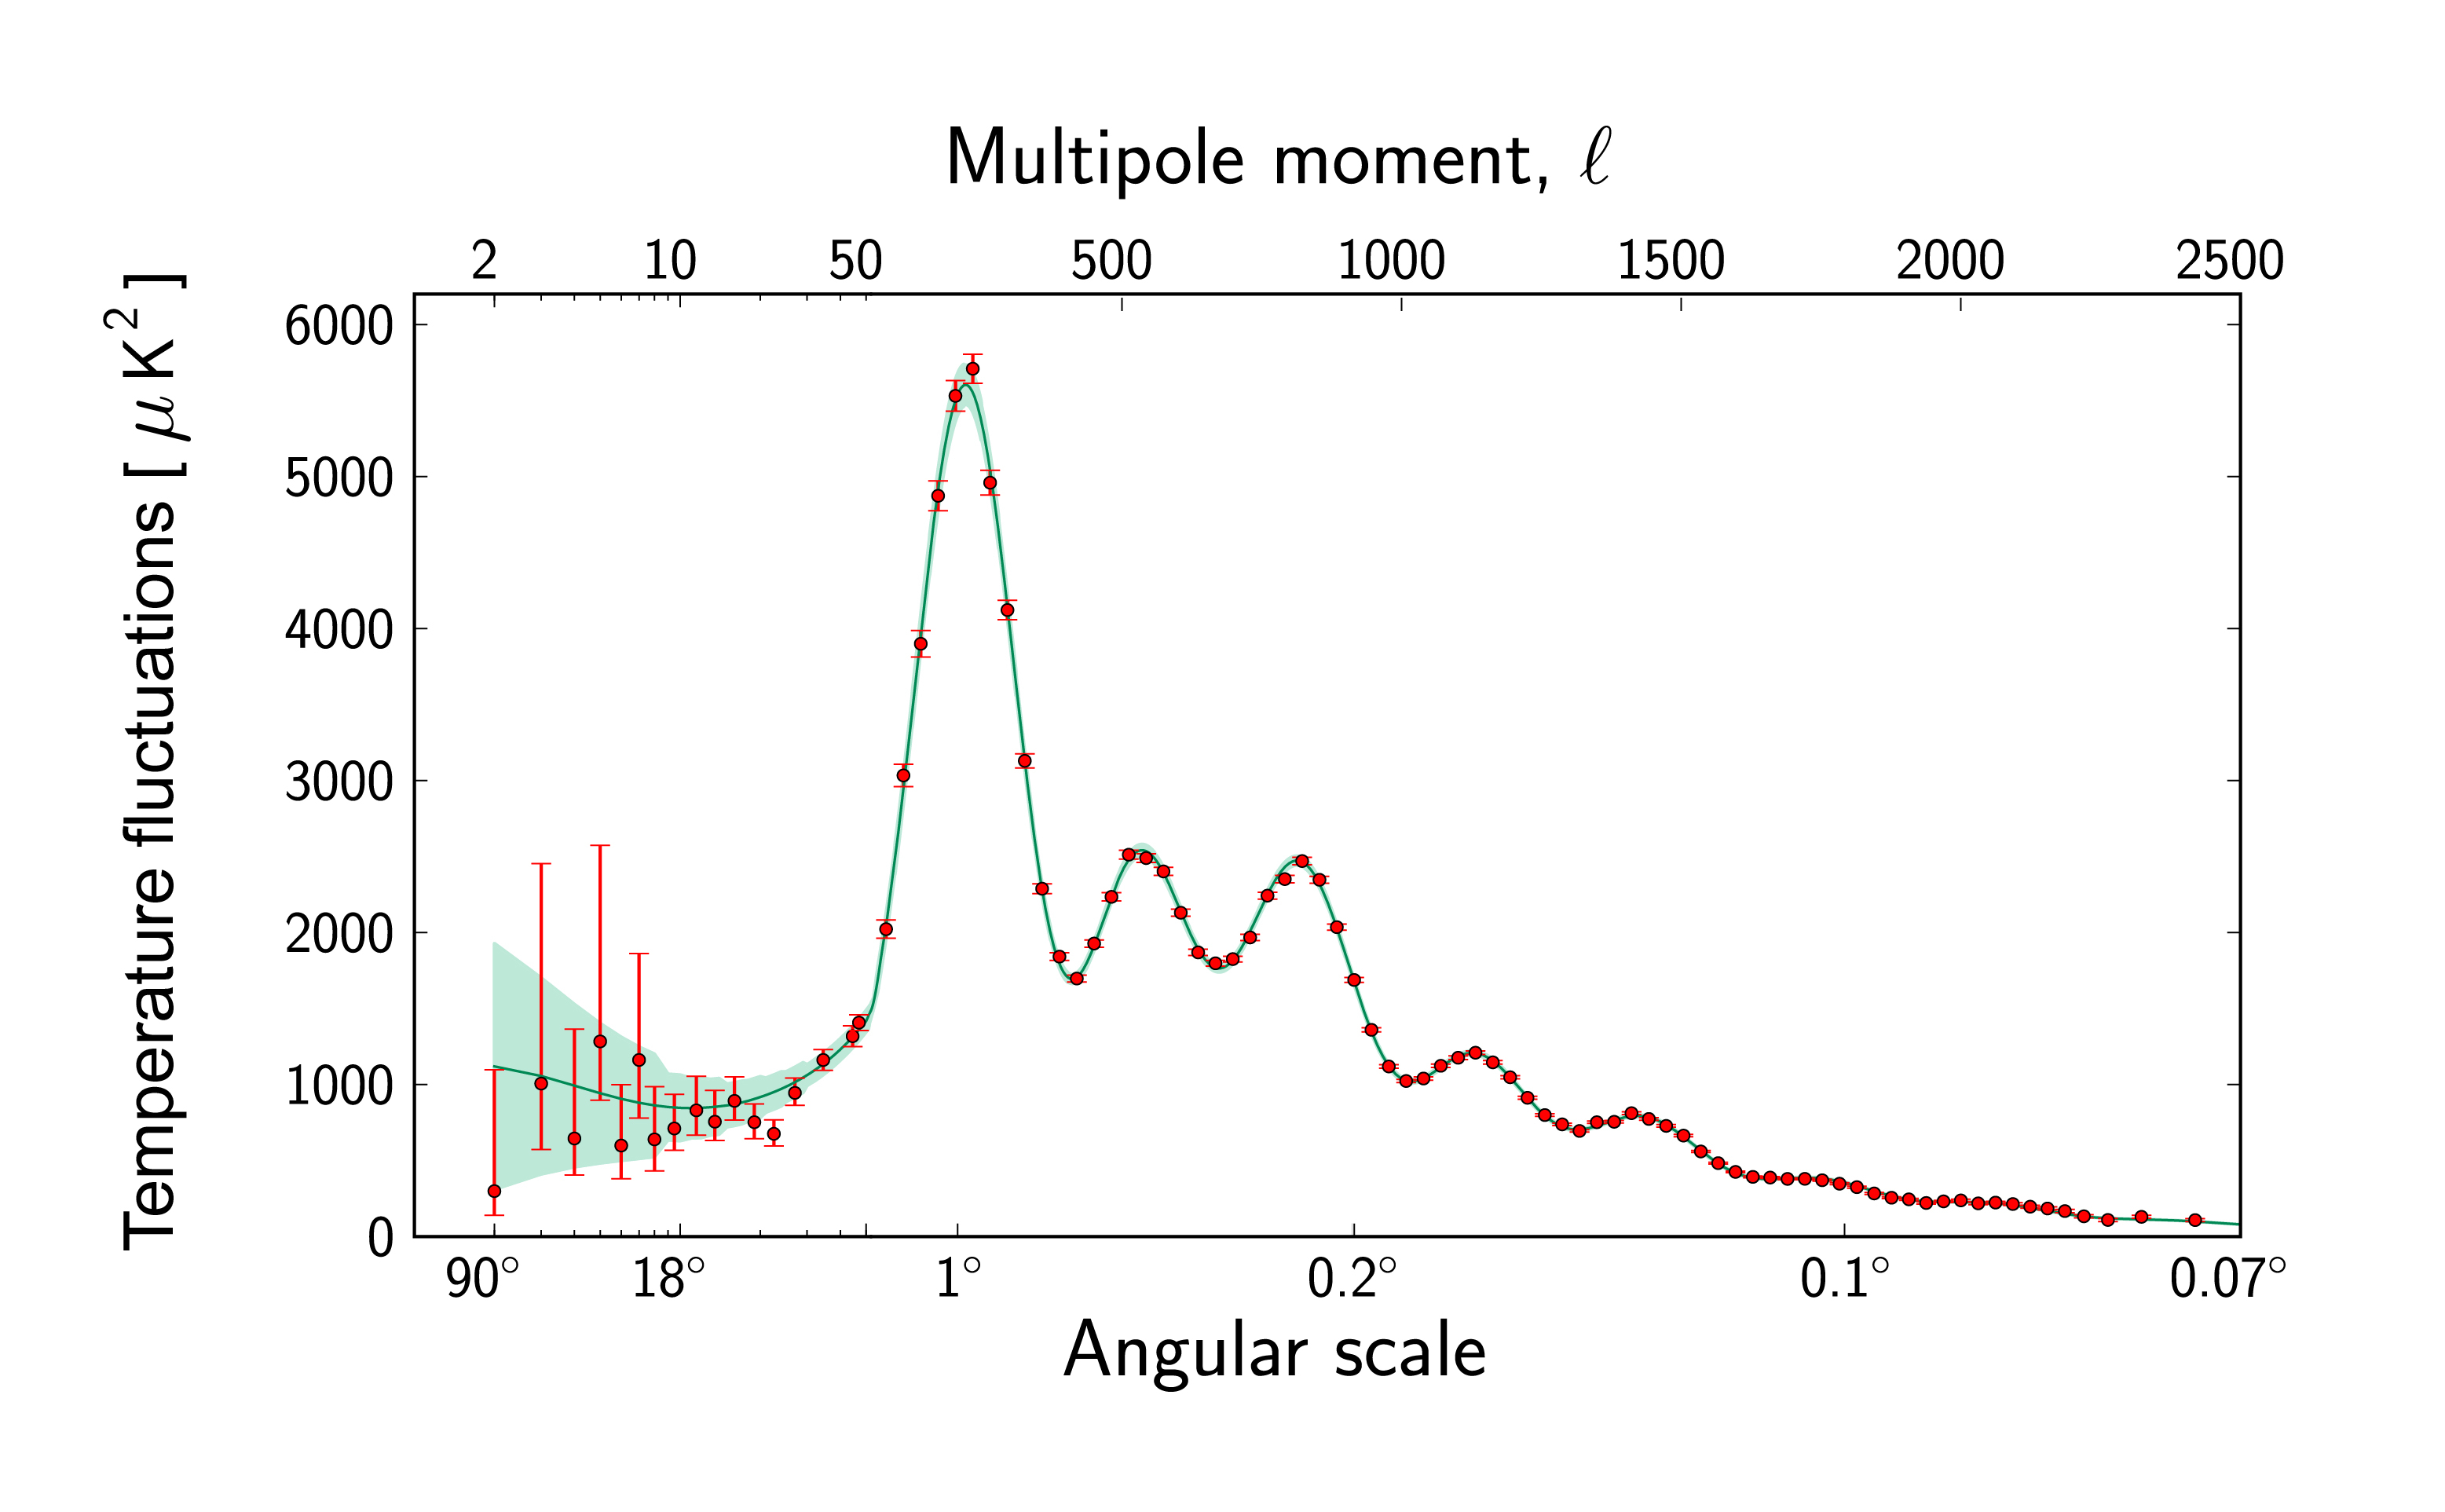
\includegraphics[width=\textwidth]{figures/Planck_power_spectrum.jpg}
    \caption{Angular Power Spectrum of Cosmic Microwave Background Temperature Fluctuations as a function of the multipole moment (\( \ell \)) and the corresponding angular scale. The observational data are depicted by red markers with associated error bars, whereas the theoretical prediction derived from the \(\Lambda\)CDM cosmological model is represented by the green curve \citep{2014A&A...571A..15P}. The primordial fluctuations imprinted at large angular scales (\( \ell \lesssim 30 \)).
    }
    \label{fig:cmb_power_spectrum}
\end{figure}

\subsection{Primodial Power Spectrum}
The standard single-field slow-roll inflation model predicts that the primordial fluctuations are nearly scale-invariant and Gaussian. The power spectrum of these primordial curvature perturbations is described by a nearly scale-invariant power-law form \citep{2003moco.book.....D}:
\begin{equation}
    P_p(k) = A_s \left(\frac{k}{k_*}\right)^{n_s - 1},
\end{equation}
where $A_s$ is the amplitude of the scalar fluctuations, $k_*$ is the pivot scale, and $n_s$ is the spectral index. The observational constraints on these parameters are provided by the Planck satellite \citep{2020A&A...641A...6P}:
\begin{equation}
    A_s = (2.101^{+0.031}_{-0.034}) \times 10^{-9}, \quad n_s = 0.965 \pm 0.004.
\end{equation}
for the pivot scale \( k_* = 0.05 \, \text{Mpc}^{-1} \).

As the universe evolves, various physical processes, such as radiation pressure, baryon-photon interactions, and dark matter dynamics, influence the growth of these initial perturbations. These effects are encapsulated in the transfer function $T(k)$, which modifies the primordial power spectrum to give the linear matter power spectrum at redshift $z$ \citep{2003moco.book.....D}:
\begin{equation}
    P(k, z) = P_p(k) T^2(k) D^2(z),
\end{equation}
where $D(z)$ is the linear growth factor that describes the growth of perturbations in the linear regime, where each $k$-mode evolves independently of the others. The growth factor is given by:
\begin{equation}
    D(a) = \frac{5 \Omega_m a}{2} \int_0^1 \frac{dx}{(\Omega_m / x + \Omega_\Lambda x^2 + 1 - \Omega_m - \Omega_\Lambda)^{3/2}},
\end{equation}
where at the limit $a \to 0$, $D(a) \to a$. 

The shape of $T(k)$ is determined by the Einstein-Boltzmann equations of a mixture of various energy components. Thus, there is no exact analytical form for $T(k)$; instead, it is typically computed using numerical codes such as \texttt{CAMB} \citep{2000ApJ...538..473L} and \texttt{CLASS} \citep{2011JCAP...07..034B}.

Qualitatively, the transfer function behaves differently on scales relative to
the equality scale \( k_{\text{eq}} \).
Since in the radiation-dominant era, the growth of perturbations on super-horizon scales is suppressed compard to those on sub-horizon scales. In the matter-dominant era, the growth of perturbations is the same on super-horizon and sub-horizon scales. Due to this, the transfer function behaves as:
\begin{equation}
    T(k) \propto 
    \begin{cases}
        1 & \text{for } k \ll k_{\text{eq}}, \\
        k^{-2} & \text{for } k \gg k_{\text{eq}}.
    \end{cases}
\end{equation}
Figure~\ref{fig:linear_power_spectrum} shows the linear matter power spectrum computed using the \texttt{CLASS} code. It is clear that the scaling of the linear power spectrum changes around $k_{\text{eq}}$. The wiggles around \( k \sim 0.1\, h/\text{Mpc} \) are due to Baryon Acoustic Oscillations (BAOs) imprinted.
\begin{figure}[ht]
    \centering
    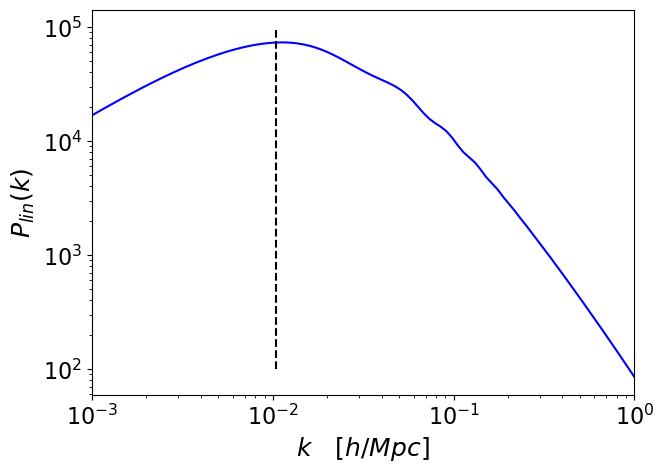
\includegraphics[width=0.8\textwidth]{figures/class.png}
    \caption{The linear matter power spectrum as a function of the wavenumber \( k \) computed using the \texttt{CLASS} code. The transition from the radiation-dominated to the matter-dominated era is evident around \( k_{\text{eq}} = 0.0104\, h/\text{Mpc} \) \citep{2020A&A...641A...6P}.
    }
    \label{fig:linear_power_spectrum}
\end{figure}

\subsection{Baryon Acoustic Oscillations}
BAOs serve as a standard ruler for cosmological distance measurements and are crucial for constraining cosmological parameters. These features originate from the oscillatory behavior of the photon-baryon plasma in the primordial universe prior to the epoch of recombination. During this period, photons and baryons are tightly coupled, effectively forming a coherent photon-baryon fluid. The coupling between photons and baryons is quantitatively characterized by the baryon-to-photon momentum density ratio, \( R \), defined as:
\begin{equation}
    R = \frac{\Pi_b}{\Pi_\gamma} = \frac{\rho_b \mathbf{v}_b}{\left(1 + \frac{1}{3}\right) \rho_\gamma \mathbf{v}_\gamma} = \frac{3 \rho_b}{4 \rho_\gamma},
\end{equation}
where \( \rho_b \) and \( \rho_\gamma \) denote the baryon and photon energy densities, respectively, while \( \mathbf{v}_b \) and \( \mathbf{v}_\gamma \) represent their respective velocities. 

The propagation of acoustic waves within the photon-baryon plasma is governed by the effective sound speed, \( c_s \), which arises from the interplay between radiation pressure and gravitational infall. The effective sound speed is derived from the effective pressure and energy density of the photon-baryon fluid:
\begin{eqnarray}
    c_s^2 &=& \frac{\partial p_\mathrm{eff}}{\partial \rho_\mathrm{eff}} = \frac{\partial p_\gamma}{\partial (\rho_b + \rho_\gamma)} \nonumber \\
    &=& \frac{1}{1 + R} \frac{\partial p_\gamma}{\partial \rho_\gamma} = \frac{1}{1 + R} \cdot \frac{1}{3} \nonumber \\
    c_s &=& \frac{1}{\sqrt{3(1 + R)}},
\end{eqnarray}
where \( p_\gamma \) and \( \rho_\gamma \) are the photon pressure and energy density, respectively. 

The acoustic oscillations in the photon-baryon plasma can be described by solutions to the linearized perturbation equations (Eq.~\eqref{eq:delta_oscillatory_mode}; we will discuss in the next section). 
e find that the perturbations in the photon density, \( \delta_\gamma \), exhibit harmonic oscillations with a wavenumber \( k \) and phase constant \( \phi \):
\begin{equation}
\delta_\gamma(k, t) \propto \cos(k c_s t + \phi),
\label{eq:gamma_oscillations}
\end{equation}
where \( \phi \) is a phase constant. Solutions of this form describe sound waves, propagating through the photon-baryon fluid.

\section{The linear evolution of density fluctuations}
Density fluctuations arise from quantum fluctuations during inflation and grow under the influence of gravity. 
Starting from the continuity and Euler equations, which govern the conservation of mass and momentum, respectively:
\begin{eqnarray}
    \label{eq:continuity_equation}
    \dfrac{\partial \rho}{\partial t} + \nabla \cdot (\rho \boldsymbol{v}) &=& 0, \\[2ex]
    \label{eq:euler_equation}
    \dfrac{\partial \boldsymbol{v}}{\partial t} + (\boldsymbol{v} \cdot \nabla) \boldsymbol{v} &=& -\dfrac{\nabla P}{\rho} - \nabla \Phi,
\end{eqnarray}
where \( \rho \) is the density, \( \boldsymbol{v} \) is the peculiar velocity field, \( P \) is the pressure, and \( \Phi \) is the gravitational potential.

To analyze perturbations in an expanding universe, we move to comoving coordinates and express the density as a perturbation around the mean density, \( \rho = \bar{\rho}(1 + \delta) \), where \( \delta \) is the density contrast. The continuity and Euler equations then become:
\begin{eqnarray}
    \label{eq:continuity_equation_rewritten}
    \dfrac{\partial \delta}{\partial t} + \dfrac{1}{a} \nabla \cdot \left( (1 + \delta) \boldsymbol{v} \right) &=& 0, \\[2ex]
    \label{eq:euler_equation_rewritten}
    \dfrac{\partial \boldsymbol{v}}{\partial t} + H \boldsymbol{v} + \dfrac{1}{a} (\boldsymbol{v} \cdot \nabla) \boldsymbol{v} &=& -\dfrac{\nabla \delta P}{a \bar{\rho} (1 + \delta)} - \dfrac{1}{a} \nabla \Phi,
\end{eqnarray}
where \( a(t) \) is the scale factor, and \( H = \dot{a}/a \) is the Hubble parameter.

To derive the equation of motion for the density contrast, we linearize the above equations under the assumption that \( \delta \ll 1 \) and \( \boldsymbol{v} \) is small. Neglecting higher-order terms in \( \delta \) and \( \boldsymbol{v} \), we obtain the linearized equations:
\begin{eqnarray}
    \label{eq:linear_continuity}
    \dfrac{\partial \delta}{\partial t} + \dfrac{1}{a} \nabla \cdot \boldsymbol{v} &=& 0, \\[2ex]
    \label{eq:linear_euler}
    \dfrac{\partial \boldsymbol{v}}{\partial t} + H \boldsymbol{v} &=& -\dfrac{\nabla \delta P}{a \bar{\rho}} - \dfrac{1}{a} \nabla \Phi.
\end{eqnarray}
The gravitational potential \( \Phi \) is related to the density contrast via Poisson's equation in comoving coordinates:
\begin{equation}
    \label{eq:poisson_equation}
    \nabla^2 \Phi = 4\pi G \bar{\rho} a^2 \delta,
\end{equation}
where \( G \) is the gravitational constant.
Assuming adiabatic perturbations, the pressure perturbation is related to the density perturbation by \( \delta P = c_s^2 \delta \rho = c_s^2 \bar{\rho} \delta \), where \( c_s \) is the sound speed.

Taking the time derivative of the linearized continuity equation (\ref{eq:linear_continuity}) and substituting the divergence of \( \boldsymbol{v} \) from the linearized Euler equation (\ref{eq:linear_euler}), we obtain:
\begin{equation}
    \dfrac{\partial^2 \delta}{\partial t^2} + 2H \dfrac{\partial \delta}{\partial t} - \dfrac{c_s^2}{a^2} \nabla^2 \delta = 4\pi G \bar{\rho} \delta.
\end{equation}
Transforming to Fourier space, where \( \nabla^2 \delta \rightarrow -k^2 \tilde{\delta}(k, t) \), the equation becomes:
\begin{equation}
    \label{eq:delta_fourier}
    \ddot{\tilde{\delta}}(k, t) + 2H \dot{\tilde{\delta}}(k, t) + \left( \dfrac{c_s^2 k^2}{a^2} - 4\pi G \bar{\rho} \right) \tilde{\delta}(k, t) = 0,
\end{equation}
where \( \tilde{\delta}(k, t) \) is the Fourier transform of the density contrast.

Defining the effective frequency squared \( \omega^2(k, t) = 4\pi G \bar{\rho} - \dfrac{c_s^2 k^2}{a^2} \), the equation simplifies to:
\begin{equation}
    \ddot{\tilde{\delta}}(k, t) + 2H \dot{\tilde{\delta}}(k, t) - \omega^2(k, t) \tilde{\delta}(k, t) = 0.
\end{equation}
The solutions to this differential equation depend on the sign of \( \omega^2(k, t) \):
\begin{itemize}
    \item \textbf{Gravity-Dominated Regime (\( \omega^2(k, t) > 0 \))}: For large-scale perturbations where gravity overcomes pressure forces (i.e., small \( k \)), the solutions are exponential:
    \begin{equation}
        \label{eq:delta_growing_mode}
        \tilde{\delta}(k, t) = C_1 e^{\lambda t} + C_2 e^{-\lambda t},
    \end{equation}
    where \( \lambda = \sqrt{\omega^2(k, t)} \). The growing mode (\( e^{\lambda t} \)) leads to the amplification of perturbations and structure formation, while the decaying mode (\( e^{-\lambda t} \)) becomes negligible over time.
    \item \textbf{Pressure-Dominated Regime (\( \omega^2(k, t) < 0 \))}: For small-scale perturbations where pressure resists gravitational collapse (i.e., large \( k \)), the solutions are oscillatory:
    \begin{equation}
        \label{eq:delta_oscillatory_mode}
        \tilde{\delta}(k, t) = e^{-Ht} \left( C_1 \cos{\left( |\omega(k, t)| t \right)} + C_2 \sin{\left( |\omega(k, t)| t \right)} \right).
    \end{equation}
    The perturbations oscillate with frequency \( |\omega(k, t)| \) and are damped by the cosmic expansion, preventing collapse on small scales.
\end{itemize}
These results illustrate the Jeans instability criterion, which states that perturbations grow only if their wavelength exceeds the Jeans length \( \lambda_J = c_s \sqrt{\dfrac{\pi}{G \bar{\rho}}} \) \citep{1902RSPTA.199....1J}.

\section{Spherical Collapse}
As gravity is attractive force, ambient matter falls into such high density regions, which results in formation of halos. 
The spherical collapse model \citep{1972ApJ...176....1G} provides a simplified description of the formation of cosmic structures by considering the evolution of a spherically symmetric overdensity in an expanding universe. Suppose that there is spherical matter around a certain point in the Universe and initial density contrast is denoted as $\delta_i \ll 1$. The equation of motion of the shell which the radius $R$ is given by:
\begin{equation}
    \ddot{R} = -\frac{GM(<R)}{R^2},
\end{equation}
where $M(<R)$ is the mass enclosed within the radius $R$. Multiplying both sides by $\dot{R}$ and integrating over time, we get:
\begin{equation}
    \dot{R}^2 = \frac{2GM(<R)}{R} + E.
\end{equation}
The constant $E$ corresponds to the energy, $E < 0$ for bound systems. From this expression, we can obtain a parametric solution for the radius $R(t)$ in term of $\theta$:
\begin{equation}
    R(t) = (GM)^{1/3} A^2 \left(1 - \cos \theta \right)
\end{equation}
\begin{equation}
    t =  A^3 \left(\theta - \sin \theta \right)
\end{equation}
where A is a constant. For a matter-dominated universe, the mean density $\bar{\rho} = (6\pi Gt^2)^{-1}$. The density contrast within the shell is given by:
\begin{equation}
    1 + \delta = \frac{\rho}{\bar{\rho}} = \frac{3M}{4\pi R^3}\, \frac{6\pi Gt^2}{M} = \frac{9}{2} \frac{\left(\theta - \sin \theta \right)^2}{\left(1 - \cos \theta \right)^3} 
\end{equation}

$\theta = \pi$ corresponds to the turnaround point, where the shell reaches its maximum radius and starts collapsing. The density contrast at the turnaround point is given by:
\begin{equation}
    \delta_{ta} = \frac{9\pi^2}{16} - 1 \approx 4.55 
\end{equation}
where the corresponding radius $R_{ta}$ and time $t_{ta}$ are:
\begin{equation}
    R_{ta} =  2(GM)^{1/3}A^2, \quad t_{ta} = \pi A^3
\end{equation}

At $\theta = 2\pi$, the shell reaches a singularity where the radius $R$ goes to zero and the density contrast $\delta$ diverges. However, in reality, this does not occur because the shell undergoes virialization and forms a halo. We assume the shell virializes at $R = R_{\text{ta}}/2$ at time $t = t_{\text{coll}}$. The density contrast at virialization is given by:
\begin{equation}
    \delta_{\text{coll}} = \delta_{\text{ta}} \times 4 \times 2^3 = 18\pi^2.
\end{equation}

In the early epoch ($\theta \ll 1$), the density contrast follows the linear theory. If we expand the density contrast and time around $\theta = 0$, we get:
\begin{equation}
    \delta = \frac{3}{20} \theta^2 + \mathcal{O}(\theta^4), \quad t = \frac{A^3}{6} \theta^3 + \mathcal{O}(\theta^5)
\end{equation}
This yields $\delta \propto t^{2/3}$, which is consistent with linear theory. Denoting this linear fluctuation as $\delta_L(t)$:
\begin{equation}
    \delta_L(t) = \frac{3(6t)^{2/3}}{20A^2}
\end{equation}
Substituting $t = t_{\text{ta}}$ and $t = t_{\text{coll}}$, we obtain:
\begin{equation}
    \delta_L(t_{\text{ta}}) = \frac{3(6\pi)^{2/3}}{20} \approx 1.06, \quad \delta_L(t_{\text{coll}}) = \frac{3(12\pi)^{2/3}}{20} \approx 1.69.
\end{equation}
Therefore, when the linear density contrast exceeds $\delta_L \approx 1.69$, the shell virializes and forms a halo.

\section{Dark Matter Halo}
\label{sec:halo}
Dark matter halos are the fundamental building blocks of cosmic structures. They form through the gravitational collapse of overdense regions in the early universe and provide the potential wells in which baryonic matter accumulates to form galaxies and clusters. 

\subsection{Halo Mass Function}
The halo mass function (HMF) describes the number density of dark matter halos as a function of their mass and redshift. The Press-Schechter (PS) formalism \citep{1974ApJ...187..425P} provides an analytical approach to calculate the HMF based on the initial density field and the theory of gravitational collapse.

Let us consider the density field which follows Gaussian distribution at each position. The probability distribution function is:
\begin{equation}
    P(\delta) d \delta=\frac{1}{\sqrt{2 \pi \sigma^2}} \exp \left(-\frac{\delta^2}{2 \sigma^2}\right) d \delta
\end{equation}
where $\sigma^2$ is the variance of the density field. Supposed that the sphere of radius $R$ contains mass $M = \frac{4}{3} \pi R^3 \bar{\rho}$, where $\bar{\rho}$ is the mean density. The density contrast within this sphere is:
\begin{equation}
    \delta_M(\boldsymbol{q}, t) = \frac{3}{4\pi} \int_{|\boldsymbol{q'}-\boldsymbol{q}|<R} \delta(\boldsymbol{q'}, t) d^3 \boldsymbol{q'}
\end{equation}
This density contrast follows Gaussian distribution. The probability distribution function of the density contrast is:
\begin{equation}
    P(\delta_M) = \frac{1}{\sqrt{2\pi \sigma^2(M)}} \exp \left(-\frac{\delta_M^2}{2\sigma^2(M)}\right)
\end{equation}
The halo formation happens when the density contrast exceeds a critical value $\delta_c$. The fraction of Lagaranian volume which collapses to form halos is:
\begin{equation}
    P_{>\delta_c} = \int_{\delta_c}^{\infty} P(\delta_M) d \delta_M = \frac{1}{\sqrt{2\pi}} \int_{\delta_c/\sigma(M)}^{\infty} e^{-x^2/2} dx
    \label{eq:collapse_fraction}
\end{equation}
Thus, mass which forms dark halo with more than mass $M$ can be calculated as $\bar{\rho_0} P_{>\delta_c}$. In Press-Schechter formalism, the mass function is given by:
\begin{equation}
    n(M) M dM = 2 \bar{\rho_0} \left|\frac{P_{\delta_c}}{d\sigma(M)}\right| \left|\frac{d\sigma(M)}{dM}\right| dM
\end{equation}
Substituting Eq.~\eqref{eq:collapse_fraction} into the above equation, we obtain:
\begin{equation}
    n(M) = \sqrt{\frac{2}{\pi}} \frac{\bar{\rho_0}}{M} \frac{\delta_c}{\sigma^2(M)} \left| \frac{d\sigma}{dM} \right| e^{-\delta_c^2/2\sigma^2(M)}
\end{equation}
The mass function can be further simplified by using the relation between the variance of the density field and the linear power spectrum $P(k)$:
\begin{equation}
    \sigma^2(M) = \int \frac{d^3 k}{(2\pi)^3} P(k) W^2(kR)
\end{equation}
where $W(kR)$ is the Fourier transform of the top-hat window function:
\begin{eqnarray}
    W(kR) &=& \int d^3 x e^{i\boldsymbol{k} \cdot \boldsymbol{x}} W_R(\boldsymbol{x}) \nonumber \\
    &=& 4\pi \int_0^R x^2 dx \frac{\sin(kx)}{kx} W_R(x) \nonumber \\
    &=& \frac{3}{(kR)^3} \left[ \sin(kR) - kR \cos(kR) \right]
\end{eqnarray}
Finally, we can construct the Press-Schechter mass function only from the linear power spectrum $P(k)$.
In reality, matter collapses into halos non-spherically. One of the most popular extensions of the Press-Schechter formalism is the Sheth-Tormen mass function \citep{1999MNRAS.308..119S}, which provides a better fit to numerical simulations by incorporating ellipsoidal collapse.

\subsection{Halo Bias}
Halo bias quantifies how dark matter halos are biased tracers of the underlying matter distribution. Massive halos tend to form in regions of higher density contrast, leading to a scale-dependent and mass-dependent bias factor $b(M)$.
\citet{1996MNRAS.282..347M} proposed a simple model for halo bias based on the Press-Schechter formalism and the spherical collapse model. They derive the analytical expression for the linear halo bias, which defined as:
\begin{equation}
    b_h(M, z) := \frac{\delta_h(M, z)}{\delta_m}
\end{equation}
where $\delta_h(M, z)$ is the overdensity of halos of mass $M$ at redshift $z$, and $\delta_m$ is the overdensity of the matter field. In the lowest-order approximation, the linear halo bias is given by:
\begin{equation}
    b_h(M, z) = 1 + \frac{\nu(M, z)^2 - 1}{\delta_c}
\end{equation}
where $\nu(M, z) = \delta_c / \sigma(M, z)$ is the peak height, and $\delta_c$ is the critical density contrast for collapse. It is then extended by \citet{2001MNRAS.323....1S} to include ellipsoidal collapse.

\subsection{Halo Density Profile}
Since halos undergo nonlinear gravitational evolution, their density profiles need numerical simulations to be determined. The most widely used model is the Navarro-Frenk-White (NFW) profile \citep{1996ApJ...462..563N, 1997ApJ...490..493N}, which is found universally in numerical simulations. The NFW profile is given by:
\begin{equation}
    \rho_\text{NFW}(r) = \frac{\rho_s}{(r/r_s)(1 + r/r_s)^2}
\end{equation}
where $\rho_s$ and $r_s$ are the characteristic density and scale radius, respectively. At large radii, the NFW profile follows a power-law behavior $\rho_{NFW} \propto r^{-3}$, while at small radii, it behaves as $\rho_{NFW} \propto r^{-1}$. The enclosed mass is not well defined for the NFW profile, so the virial radius $r_{\text{vir}}$ and $r_{200c}$, which encloses a density contrast of 200 times the critical density, are used instead.

After specifying the boundary, one can compute the halo mass as \citep{2011MNRAS.414.1851O}:
\begin{equation}
    M_{\text{vir}} = 4\pi r_s^3 \rho_s m(c_{\text{vir}})
\end{equation}
with
\begin{equation}
    m(c) = \int_0^{c} \frac{x dx}{(1 + x)^2} = \ln(1 + c) - \frac{c}{1 + c}
\end{equation}
where $c_{\text{vir}} = r_{\text{vir}}/r_s$ is the concentration parameter. 

Another widely used profile is the Einasto profile \citep{1965TrAlm...5...87E}, which provides a better fit to numerical simulations at small radii. The Einasto profile is given by:
\begin{equation}
    \rho_{\text{Ein}}(r) = \rho_s \exp \left( -\frac{2}{\alpha} \left[ \left( \frac{r}{r_s} \right)^\alpha - 1 \right] \right)
\end{equation}
where $\rho_s$ and $r_s$ are the characteristic density and scale radius, respectively, and $\alpha$ is the shape parameter. 